\documentclass[12pt]{article}
\usepackage[utf8]{inputenc}
\usepackage{amsmath}
\usepackage{bm}
\usepackage{graphicx}
\graphicspath { {./images/} }
\title{2DV513 Assignment 2}
\author{Jacob Skoog \\ js224wv}
\begin{document}

\begin{titlepage}
\maketitle
\end{titlepage}

\section {Relational Algebra}\label{sec:relational-algebra}

\subsection {Names of students in 1dv513}\label{subsec:names-of-students-in-1dv513}
\begin {math}
ids = \Pi\_{id}(\sigma\_{code=1dv513}(enrolled))
\end {math}
\\
\begin {math}
answer = \Pi\_{name}(\sigma\_{id \in ids}(student))
\end {math}

\subsection {Names of students in both 1dv513 and 2dv513}\label{subsec:names-of-students-in-both-1dv513-and-2dv513}
\begin {math}
ids1dv513 = \Pi\_{id}(\sigma\_{code=1dv513}(enrolled))
\end {math}
\\
\begin {math}
ids2dv513 = \Pi\_{id}(\sigma\_{code=1dv513}(enrolled))
\end {math}
\\
\begin {math}
union = ids1dv513 \cup ids2dv513
\end {math}
\\
\begin {math}
intersection = ids1dv513 \cap ids2dv513
\end {math}

\paragraph{If} interpreted as a union of students in 1dv513 and 2dv513:
\begin {equation}
\Pi_{name}(\sigma_{id \in union}(student))\label{eq:equation1}
\end {equation}

\paragraph{If} interpreted as an intersection of students in both 1dv513 and 2dv513:
\begin {equation}
\Pi_{name}(\sigma_{id \in intersection}(student))\label{eq:equation2}
\end {equation}

\subsection {Who teaches 2dv610}\label{subsec:who-teaches-2dv610}
\begin{math}
\Pi\_{lecturer} (\sigma\_{code=2dv610}(subject))
\end{math}

\subsection {Who teaches 1dv513 and 2dv513}\label{subsec:who-teaches-1dv513-and-2dv513}

\paragraph{If} intepreted as unions of teachers of both 1dv513 and 2dv513:
\begin {equation}
\Pi_{lecturer} (\sigma_{code=1dv513}(subject) \cup \sigma_{code=2dv513}(subject))\label{eq:equation3}
\end {equation}
\paragraph{If} interpreted as the intersection of those teaching in both 1dv513 and 2dv513:
\begin {equation}
\Pi_{lecturer} (\sigma_{code=1dv513}(subject) \cap \sigma_{code=2dv513}(subject))\label{eq:equation4}
\end {equation}

\subsection {Names of students *not* taught by Ilir}\label{subsec:names-of-students-*not*-taught-by-ilir}

\begin {math}
codes = \Pi\_{code}(\sigma\_{lecturer=Ilir}(subject))
\end{math}
\\
\begin {math}
IlirStudents = \Pi\_{id}(\sigma\_{code \in codes}(enrolled))
\end {math}
\\
\begin {math}
answer = \Pi\_{name}(\sigma\_{id \notin IlirStudents}(student))
\end {math}

\section {FDs and Normalisation}\label{sec:fds-and-normalisation}
\subsection {Functional Dependencies}\label{subsec:functional-dependencies}

\begin {figure}[h]
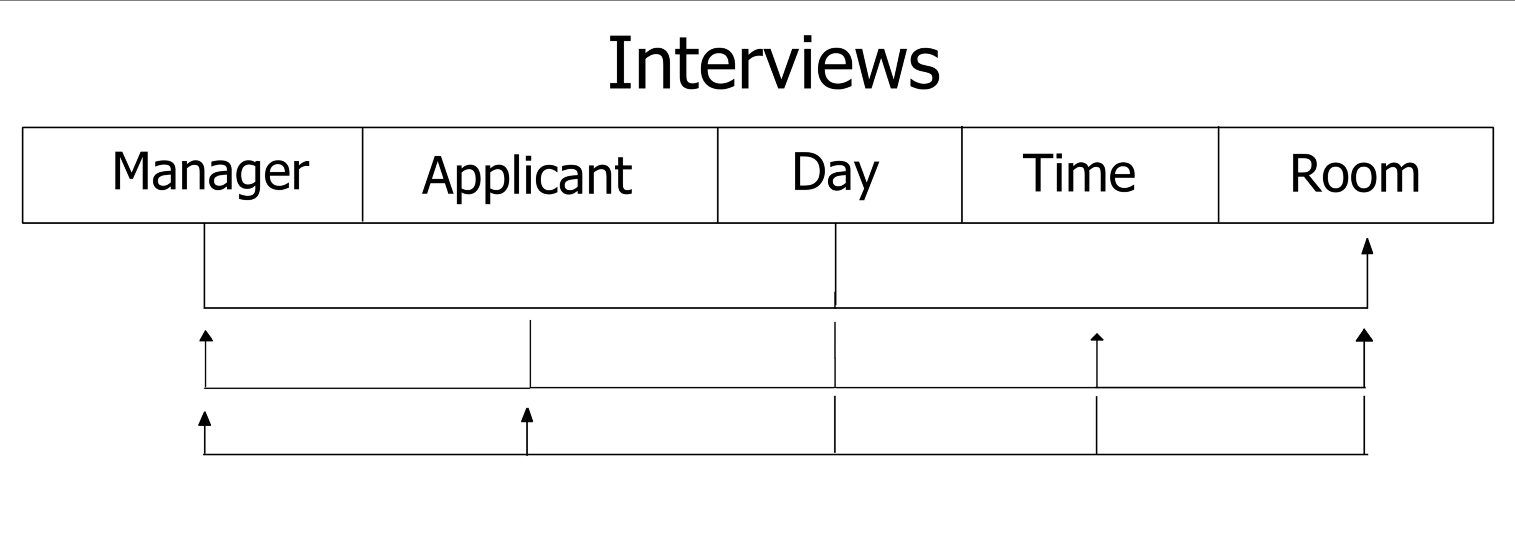
\includegraphics [width=\textwidth]{FD}
\caption { The functional dependencies of the Interviews Relation	}
\label{fig:fd1}
\end {figure}

As can be seen in figure~\ref{fig:fd1}, three functional dependencies have been identified.

\subsubsection {\(\{Manager, Day\} \mapsto \{Room\}\)}
Since a manager is only in a single room in any set day, you can determine the room from the Manager and Day attributes.

\subsubsection {\(\{Applicant, Day\} \mapsto \{Manager, Time, Room\}\)}
As an applicant will only have a single interview in a set day, and a single interview will have a single manager, at a single time, at a single room, this dependency holds.

\subsubsection {\(\{Day, Time, Room\} \mapsto \{Manager, Applicant\}\)}
If day, time, and room are known they will identify a unique interview, which will have a single manager and applicant.

\subsection {The keys of the relation}\label{subsec:the-keys-of-the-relation}

\subsubsection {Candidate Keys}

Since \(\{Applicant, Day\} \mapsto \{Manager, Time, Room\}\) (1) and \(\{Day, Time, Room\} \mapsto \{Manager, Applicant\}\) (2) will both identify a single unique tuple in R, they are candidate keys. \\
As the choice of primary key is arbitrary at this point, I will choose (1) as the primary key and (2) as the secondary key.

\subsection {3NF but not BCNF}\label{subsec:3nf-but-not-bcnf}
\subsubsection {1NF}

All the values are atomic, so the relation is 1NF\@.

\subsubsection {2NF}

The only non-prime attribute is 'Manager'.

The relation is 2NF as Manager is functionally dependent on the chosen primary key (and the secondary key).
The functional dependency is furthermore full, as the removal of any attribute would break the functional dependency.
The same is also true of the secondary key.

\subsubsection {3NF}

As stated when discussing 2NF, the only non-prime attribute is 'Manager', and Manager is not functionally dependent on any other non-prime attribute, as there is no other non-prime attribute.
Or, to use the general defenition of 3NF:\\
There are three non-trivial functional dependencies in the relation.
Two of these are superkeys of the relation (fulfilling clause (a) of the general definition).
The only FD \(X \mapsto A\) where X is not a superkey is the FD \(\{Manager, Day\} \mapsto \{Room\}\), and here A is a prime attribute \{Room\}, thus fullfilling clause (b).
\\Thus, the relation is 3NF\@.

\subsubsection {BCNF}
As mentioned above, one of the functional dependencies fulfilled clause (b) of 3NF, but that clause is not allowed in BCNF. The relation is therefore not in BCNF\@.

\subsection {Decompose into BCNF}\label{subsec:decompose-into-bcnf}

The decomposition must pass the non-additive join test.
I propose the following decomposition: \(R_1(Manager, Day, Room), R_2(Manager, Applicant, Day, Time)\)\\
Then, \(R_1 \cap R_2 = \{Manager, Day\}, R_1 - R_2 = \{Room\}, and \{Manager, Day\} \mapsto \{Room\} \in F^+\), thus this decomposition passes the test.

\begin {figure}[h]
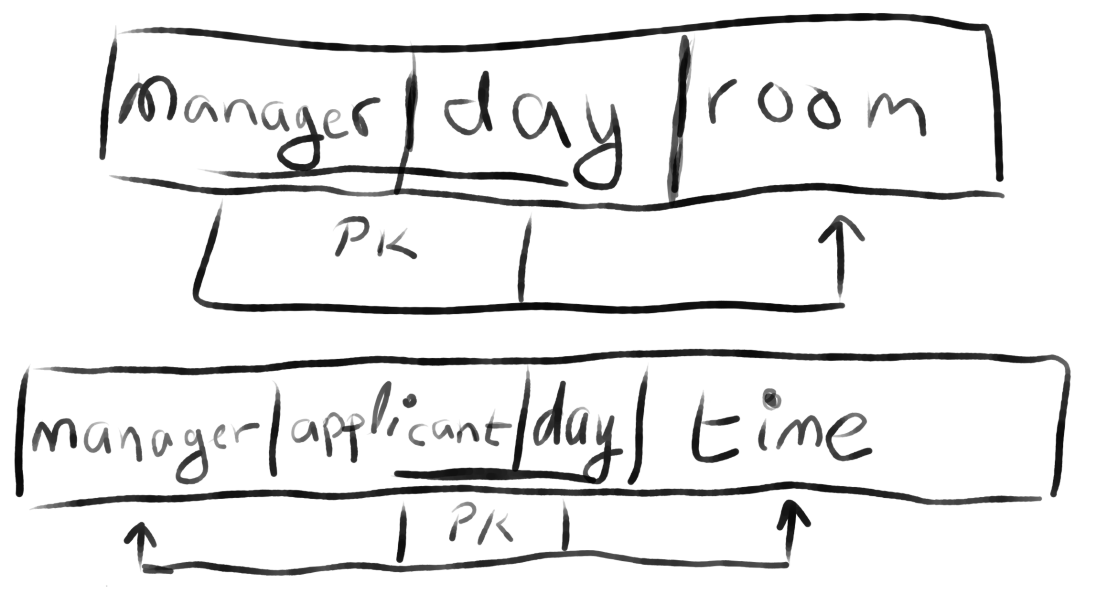
\includegraphics[width=\textwidth]{BCNF}
\caption{The two decomposed relations and their functional dependencies}\label{fig:ER}
\end {figure}

As can be seen on the diagram~\ref{fig:ER}, the two relations are now BCNF-compliant, as now whenever an FD \(X \mapsto A\) holds, X is a superkey (as neither of the keys above can lose any attribute).

\subsection {ER Diagram}\label{subsec:er-diagram}
\begin {figure}[h]
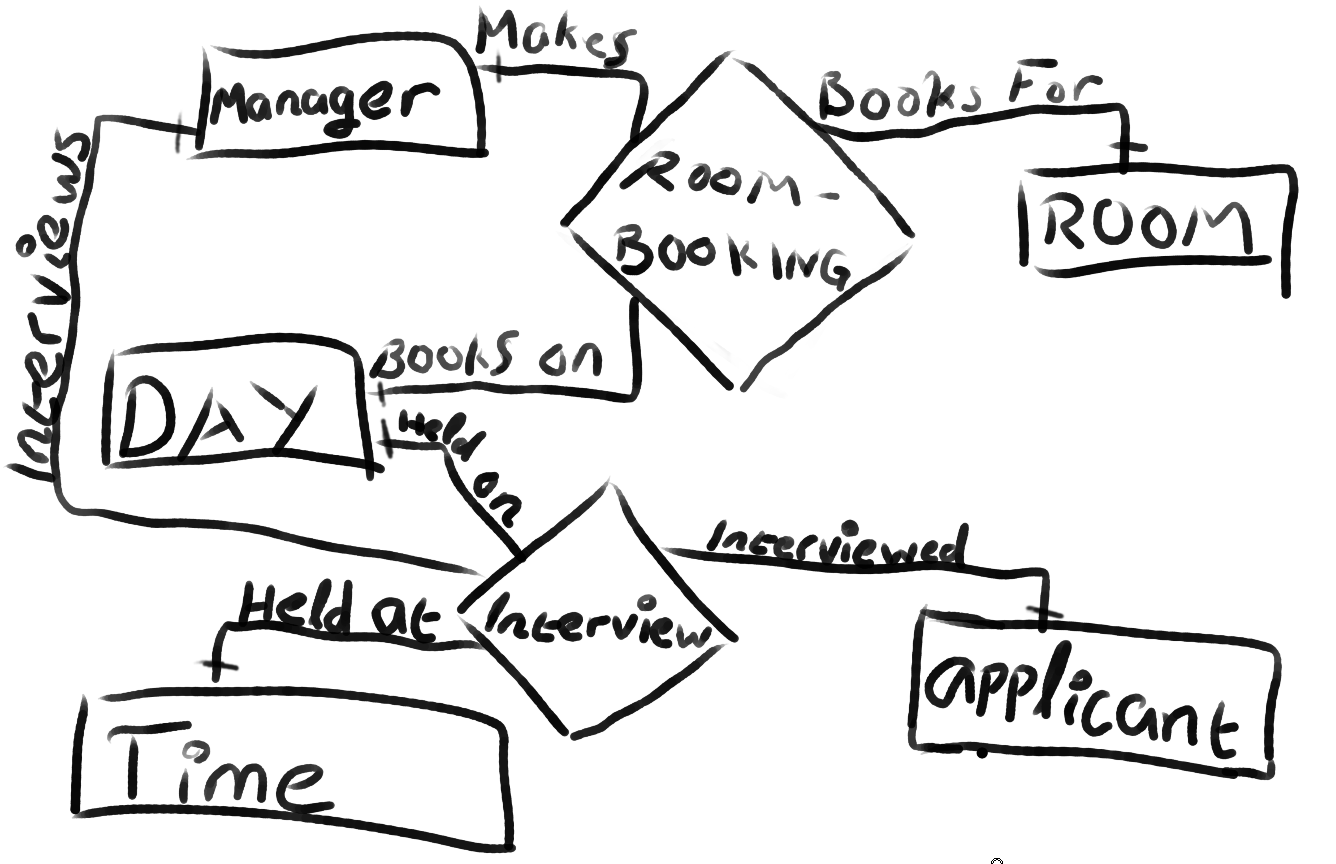
\includegraphics[width=\textwidth]{ER}
\caption {Entity Relation Diagram for the Relation}\label{fig:figure2}
\end {figure}

\section {Setting up the reddit database}\label{sec:setting-up-the-reddit-database}
\section {Importing the data}\label{sec:importing-the-data}
\section {SQL Queries}\label{sec:sql-queries}
\end{document}